\documentclass[nobib]{tufte-handout}


\usepackage{ifluatex, ifxetex} % проверка, как компилируется файл

% black magic!
% solving problem with tufte-handout + xelatex
% http://tex.stackexchange.com/questions/200722/
% https://tex.stackexchange.com/questions/47576/
\ifx\ifxetex\ifluatex\else % если xelatex или lualatex
  \newcommand{\textls}[2][5]{%
    \begingroup\addfontfeatures{LetterSpace=#1}#2\endgroup
  }
  \renewcommand{\allcapsspacing}[1]{\textls[15]{#1}}
  \renewcommand{\smallcapsspacing}[1]{\textls[10]{#1}}
  \renewcommand{\allcaps}[1]{\textls[15]{\MakeTextUppercase{#1}}}
  \renewcommand{\smallcaps}[1]{\smallcapsspacing{\scshape\MakeTextLowercase{#1}}}
  \renewcommand{\textsc}[1]{\smallcapsspacing{\textsmallcaps{#1}}}
\fi

% с альтернативного источника:
%\ifluatex % Allow rendering with LuaTeX by setting up the spacing using fontspec features
%  \renewcommand\allcapsspacing[1]{{\addfontfeature{LetterSpace=15}#1}}
%  \renewcommand\smallcapsspacing[1]{{\addfontfeature{LetterSpace=10}#1}}
%\fi

% lua produces strange notes
% https://tex.stackexchange.com/questions/328431

\usepackage{fontspec} % работа со шрифтами
%\usepackage{polyglossia} % учим русский как иностранный :)

%\setmainlanguage{engish}
%\setotherlanguages{english}

% заменяем --- на тире, << на кавычки и т.д.:
\defaultfontfeatures{Ligatures=TeX}

% download "Linux Libertine" fonts:
% http://www.linuxlibertine.org/index.php?id=91&L=1
\setmainfont{Linux Libertine O} % or Helvetica, Arial, Cambria
% why do we need \newfontfamily:
% http://tex.stackexchange.com/questions/91507/
\newfontfamily{\cyrillicfonttt}{Linux Libertine O}
\newfontfamily{\cyrillicfont}{Linux Libertine O}
\newfontfamily{\cyrillicfontsf}{Linux Libertine O}



\usepackage{amsmath}
\usepackage{amsthm}
\usepackage{amsfonts}
\usepackage{amssymb}
\usepackage{url} % вставка \url{}
\usepackage{graphicx} % вставка графиков
\usepackage{csquotes} % адаптирующиеся кавычки командой \enquote{}
\usepackage{comment} % ingore everything between \begin{comment} \end{comment}
\usepackage{answers} % separate problems and solutions
\usepackage{tikz} % pictures with tikz language
\usepackage{todonotes} % todo in documents
\usepackage{multicol} % make several columns
\usepackage{subfigure}

\usepackage{enumitem} % для создания своих нумерующих списков (хак для гиперссылок)

%\usepackage[left=2cm,right=2cm,top=2cm,bottom=2cm]{geometry}


% very useful during de-bugging!
% \usepackage[left]{showlabels}
% \showlabels{hypertarget}
% \showlabels{hyperlink}


\DeclareMathOperator{\Var}{Var}
\DeclareMathOperator{\card}{card}
\DeclareMathOperator{\Cov}{Cov}
\DeclareMathOperator{\Corr}{Corr}
\DeclareMathOperator{\E}{E}
\renewcommand{\P}{\mathbb{P}}
\newcommand{\I}{\mathbb{I}} % индикатор события
\newtheorem{theorem}{Theorem}
\newtheorem{corollary}{Corollary}[theorem]
\newtheorem{lemma}[theorem]{Lemma}

\usepackage[bibencoding = auto, backend = biber,
sorting = none]{biblatex}

%\addbibresource{probability_dna.bib}



%\title{Geometric interpretaion of main concepts and theorems in econometrics}
\title{some title}
\author{}
\date{\today}
\begin{document}

\maketitle

%\section{Literature review}

\section{Regression}

\subsection{Correlation}

\marginnote{The most widespread definition of correlation is
\[
\Corr(X,Y)  = \frac{\Cov(X, Y)}{\sqrt{\Var(X)\Var(Y)}}
\]}

The most crucial part in defining correlation geometrically is definig the dot product as it enables to compute the length of a vecotr:
\[
|\vec{a}| = \sqrt{\langle \vec{a},  \vec{a}\rangle}
\]
and the angle between any two vectors:
\[
\cos(\vec{a}, \vec{b}) = \frac{\langle \vec{a},  \vec{a}\rangle}{|\vec{a}| |\vec{b}|}
\]
Now we define scalar product of two random vectors as covariation between them:
\[
\langle X, Y \rangle = \Cov(X, Y)
\]
The main characteristics of a random vector are its length and direction.
So, we introduce the length
\[
\sqrt{\Cov{X,X}} = \sqrt{\Var(X)} = \sigma_X
\]
and the angle between two random vectors
\[
\cos(X,Y) = \frac{\Cov(X,Y)}{\sqrt{\Var(X)\Var(Y)}} = \Corr(X,Y)
\]
Note that from the definition of the angle it follows that correlation is limited within an interval $[-1,1]$.

\begin{figure}[ht!]
\begin{center}
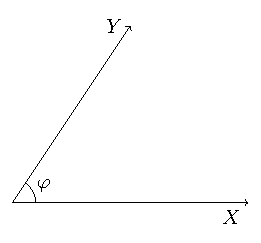
\includegraphics{images/corr_def.pdf}
\label{fig:corr_def}
\caption{Random vector $X$ of length $\sigma_X$ and random vector $Y$ of length $\sigma_Y$, $\cos \varphi$ is the angle between $X$ and $Y$.}
\end{center}
\end{figure}

Another important geometrical tool is projection. Recall that for any two vectors the scalar product $\langle \vec{a}, \vec{b} \rangle$ can be interpreted as the length of projected $\vec{b}$ multuplied by the length of $\vec{a}$.
The projection itself is $cos(\vec{a}, \vec{b}) \vec{b}$.
Same holds for random vectors. The projection of a random vector $Y$ onto $\{cX| c \in \mathbb{R}\}$ is $\Corr(X,Y) \cdot Y$.


\subsection{Regression line and point of averages}

\marginnote{
If the regression contains the intercept, the following equation holds:
\begin{align*}
\hat y  &= X \hat \beta = X (X^T X)^{-1} X^T y \\
&= X (X^T X)^{-1} X^T X \beta + X (X^T X)^{-1} X^T \varepsilon
\end{align*}
Premultiplying both sides by $X^T$, we obtain:
\begin{align*}
X^T \hat y &=  X^T X (X^T X)^{-1} X^T X \beta \\
&+ X^T X (X^T X)^{-1} X^T \varepsilon \\
&= X^T X \beta + X^T \varepsilon
\end{align*}
This is a system of equations. The first row of $X^T$ is $\mathbf{1}$ vector, so we can write out the first equation:
\[
\sum_{i=1}^n \hat y_i = \sum_{i=1}^{n} \sum_{j=1}^{k} x_{ij} \beta_{j}
\]
From the first equation in the system
\[
X^T \hat y = X^T y
\]
we obtain
\[
\sum_{i=1}^{n} \hat y_i = \sum_{i=1}^{n} y
\]
And this finishes the proof:
\[
\frac{1}{n} \sum_{i=1}^{n} y = \frac{1}{n} \sum_{i=1}^{n} \sum_{j=1}^{k} x_{ij} \beta_{j}
\]
}

\begin{theorem}
The point of averages lies on the estimated regression line.
\end{theorem}

\begin{proof}
For the geometrical proof it suffices to show that $\hat y$ is a linear combination of the regressors, which is true by construction,
and that $\frac{1}{n} \sum_{i=1}^{n} \hat y_i = \frac{1}{n} \sum_{i=1}^{n} y$. In order for the pictures to be more clear the proof will be presented for the case of two regressors.

The first step is regressing $y$ on $Lin(\mathbf{1}, x)$. As shown in Figure~\ref{fig:averages_lin}, we obtain $\hat y$ as a linear combination of $\mathbf{1}$ and $x$.
The next step is to regress both $y$ and $\hat y$ on $\mathbf{1}$ which results in $\bar y$ and $\bar \hat y$ correspondingly.
By the theorem of three perpendiculars, $\bar y = \bar \hat y$ which is shown in Figure~\ref{fig:averages_bars}.

\begin{figure}[ht!]
\begin{center}
\subfigure[]{
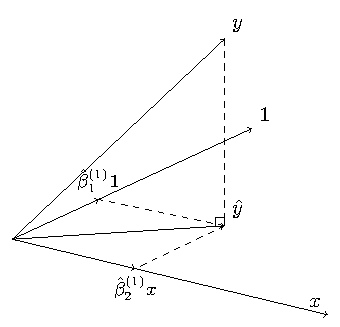
\includegraphics[width=0.4\linewidth]{images/averages_1.pdf}
%\caption{Regression of $y$ on $Lin(x,z)$} %% подпись к рисунку
\label{fig:averages_lin} }
\hspace{4ex}
\subfigure[]{
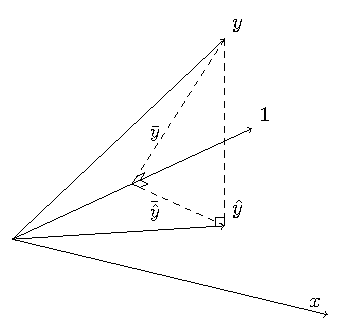
\includegraphics[width=0.4\linewidth]{images/averages_2.pdf}
%\caption{$Lin(x, z)$}
\label{fig:averages_bars}}
\caption{\subref{fig:averages_lin}: Regression of $y$ on $Lin(\mathbb{1},x)$; \subref{fig:averages_bars}: Regression of $y$ and $\hat y$ on $\mathbb{1}$.}
\end{center}
\end{figure}


\end{proof}

\subsection{Frisch–Waugh–Lovell theorem}

\marginnote{From regresison~\ref{eq:fwl_2} we get the following estimator:
\begin{align*}
\hat\beta_2 &= ((M_1 X_2)^T M_1 X_2)^{-1}(M_1 X_2)^T M_1 y \\
&= (X_2^T M_1^T M_1 X_2)^{-1}  X_2^T M_1^T M_1 y \\
&= (X_2^T M_1 X_2)^{-1}  X_2^T M_1 y
\end{align*}
As for regresison~\ref{eq:fwl_1}, let us note that due to $y = \hat y + \hat u$ $y$ can be decomposed as follows:
\[
y = Py + My = X_1 \hat \beta_1 + X_2 \hat \beta_2 + My
\]
Premultiplying both sides by $X_2^T M_1$, we obtain:
\begin{align*}
X_2^T M_1 y &= X_2^T M_1 X_1 \hat\beta_1 + X_2^T M_1 X_2 \hat\beta_2 + X_2^T M_1 M y \\
&=  X_2^T M_1 X_2 \hat\beta_2 + X_2^T M_1 M y \\
&= X_2^T M_1 X_2 \hat\beta_2
\end{align*}
On the last step we used the fact that
\begin{align*}
(X_2^T M_1 M y)^T = y^T M^T M_1^T X_2 \\
= y^T M M_1 X_2 = y^T M X_2 = 0^T
\end{align*}
Assuming $X_2^T M_1 X_2$ is invertible, we get the same estimator
\[
\hat\beta_2 = (X_2^T M_1 X_2)^{-1}  X_2^T M_1 y
\]
}

\begin{theorem}
Consider regression
\begin{equation} \label{eq:fwl_1}
y = X_1 \beta_1 + X_2 \beta_2 + u
\end{equation}
where $X_{n \times k} = [X_1 X_2]$, i.e. $X_1$ consists of first $k_1$ columns of $X$ and $X_2$ consists of remaining $k_2$ columns of $X$,
$\beta_1$ and $\beta_2$ are comfortable, i.e. $k_1 \times 1$ and $k_2 \times 1$ vectors.
Consider another regresison
\begin{equation}  \label{eq:fwl_2}
M_1 y = M_1 X_2 \beta_2 + M_1 u
\end{equation}
where $M_1 = I - P_1$ projects onto the orthogonal complement of the column space of $X_1$ and $P_1 = X_1(X_1^TX_1)^{-1}X_1^T$ is the projection onto the column space of $X_1$.
Then the estimate of $\beta_2$ from regression~\ref{eq:fwl_1} will be the same as the estimate from regression~\ref{eq:fwl_2}.
\end{theorem}

\begin{proof}
Geometrical proof will be presented for the following model:
\begin{equation} \label{eq:fwl_proof}
y_i = \beta_1 x_i + \beta_2 z_i + u_i
\end{equation}

We start with regression `all-at-once' and will distinct its coefficients with index $(1)$. The only step in obtaining $\beta_1^{(1)}$ is regressing $y$ on $Lin(x,z)$ and then expanding $\hat y$ as a linear combination of basis vectors $x$ and $z$,
which is shown in Figure~\ref{fig:fwl_1_regression_3d}. Figure~\ref{fig:fwl_1_regression_lin} depicts $Lin(x, z)$.

\begin{figure}[ht!]
\begin{center}
\subfigure[]{
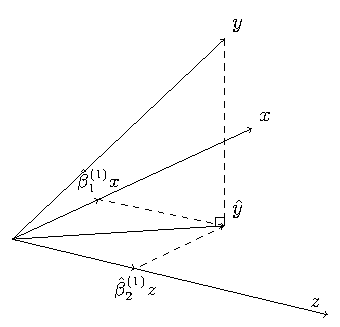
\includegraphics[width=0.4\linewidth]{images/fwl_1_regression.pdf}
%\caption{Regression of $y$ on $Lin(x,z)$} %% подпись к рисунку
\label{fig:fwl_1_regression_3d} }
\hspace{4ex}
\subfigure[]{
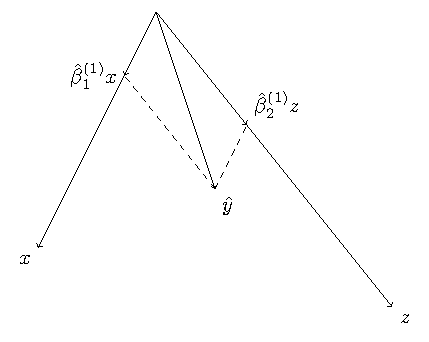
\includegraphics[width=0.4\linewidth]{images/fwl_1_regression_lin.pdf}
%\caption{$Lin(x, z)$}
\label{fig:fwl_1_regression_lin}}
\caption{\subref{fig:fwl_1_regression_3d}: Regression of $y$ on $Lin(x,z)$; \subref{fig:fwl_1_regression_lin}: $Lin(x, z)$.}
\end{center}
\end{figure}

As for the model~\ref{eq:fwl_2}, where several regressions are performed consecutively, we start with regressing $y$ on $z$, resulting in $\tilde{y}$, which we will refer to as ``cleansed'' $y$.

\begin{equation}\label{eq:fwl_2_y_clean}
\begin{aligned}
y &= \alpha z + \varepsilon \\
\hat\alpha &= \frac{y^T z}{z^T z} \\
\tilde{y} &= \hat\varepsilon = y - \frac{y^T z}{z^T z}z
\end{aligned}
\end{equation}

Following that, $x$ is regressed on $z$, resulting in $\tilde{x}$ — ``cleansed'' $x$.

\begin{equation}\label{eq:fwl_2_x_clean}
\begin{aligned}
x &= \gamma z + \nu \\
\hat\gamma &= \frac{x^T z}{z^T z} \\
\tilde{x} &= \hat\nu = x - \frac{x^T z}{z^T z}z
\end{aligned}
\end{equation}

Geometric results of these two steps are presented in~\ref{fig:fwl_2_regression_first}.

Finally, `cleansed' $y$ must be regressed on `cleansed' $x$. However, it cannot be performed immediately as $\tilde{y}$ and $\tilde{x}$ are skew lines.
So at first, we fix this problem by translation and after taht obtain $\hat\beta_1^{(2)}\tilde x$ (see Figure~\ref{fig:fwl_2_regression_trans}).

\begin{figure}[ht!]
\begin{center}
\subfigure[]{
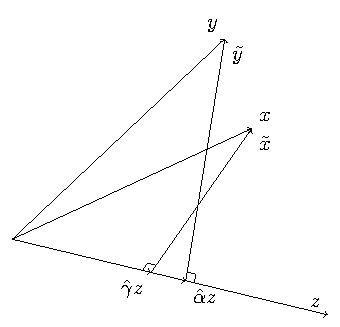
\includegraphics[width=0.4\linewidth]{images/fwl_2_regression.pdf}
%\caption{Regression of $y$ on $Lin(x,z)$} %% подпись к рисунку
\label{fig:fwl_2_regression_first} }
\hspace{4ex}
\subfigure[]{
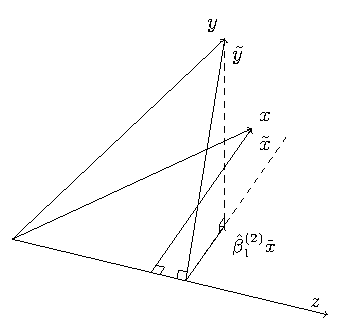
\includegraphics[width=0.4\linewidth]{images/fwl_2_regression_translation.pdf}
%\caption{$Lin(x, z)$}
\label{fig:fwl_2_regression_trans}}
\caption{\subref{fig:fwl_2_regression_first}: Regression of $y$ on $z$ and of $x$ on $z$; \subref{fig:fwl_2_regression_trans}: Translation of $\tilde{x}$.}
\end{center}
\end{figure}

Now, let us picture all the results in one figure and mark some main points.

\begin{figure}[ht!]
\begin{center}
\subfigure[]{
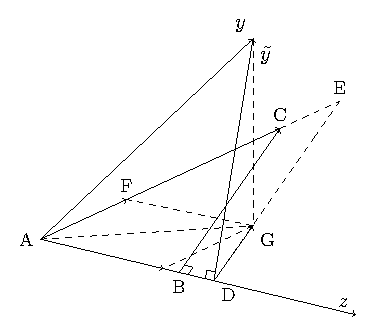
\includegraphics[width=0.4\linewidth]{images/fwl_3_3d.pdf}
%\caption{Regression of $y$ on $Lin(x,z)$} %% подпись к рисунку
\label{fig:fwl_3_3d} }
\hspace{4ex}
\subfigure[]{
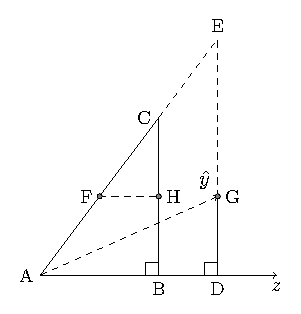
\includegraphics[width=0.4\linewidth]{images/fwl_3_lin.pdf}
%\caption{$Lin(x, z)$}
\label{fig:fwl_3_lin}}
\caption{\subref{fig:fwl_3_3d}: Point A stands for the origin, B — $\hat\gamma z$, C — $x$, D — $\hat\alpha z$, E — intersection of vector $x$ and line parallel to $\tilde x$,
F — $\hat\beta_1^{(1)} x$, G — $\hat\beta_1^{(2)} \tilde{x}$; \subref{fig:fwl_3_lin}: $Lin(x,z)$.}
\end{center}
\end{figure}

In Figure~\ref{fig:fwl_3_lin} segments AF and BH = DG stand for $\hat\beta_1^{(1)}x$ and $\hat\beta_1^{(2)}\tilde x$ respectively,
while segments AC and BC represent $x$ and $\tilde{x}$. Having two congruent angles, triangles ABC and FHC are simillar.
Then, it follows:
\[
\frac{AF}{AC} = \frac{BH}{BC} \Leftrightarrow \frac{\hat\beta_1^{(1)}x}{x} = \frac{\hat\beta_1^{(2)}\tilde x}{\tilde x} \Leftrightarrow \hat\beta_1^{(1)} = \hat\beta_1^{(2)}
\]
\end{proof}


%\section{Geometric properties of distributions}

%\section{Partial correlation}


\end{document}
